\thispagestyle{empty}

\vspace*{-10mm}

\begin{center}
    {\Large \bf \cvut\\[2mm] \fjfi\\ }
    \vspace{3mm}
    
    {\large \bf \kdaiz}\\
     \vspace{2mm}  
%    {\bf Obor: \obor}\\
   
   \vspace{0mm}

\begin{figure}[h]
\begin{center}
	
\includegraphics[scale=1.5]{cvut.jpg}
\end{center}
\end{figure}

    \vspace{5mm}

%   {\LARGE \bf \nazevcz\vspace{8mm}\par  \Large \nazeven}

   \vspace{0mm}
   {\Huge\textbf{\MakeUppercase{\typprace}}}

   \vspace{15mm}
   {\Large \textbf{\nazevcz}}
   
\end{center}

   \vfill
   {\large
    \begin{tabular}{ll}
    Autor: & \autor\\
    Vedoucí: & \vedouci\\
    Akademický rok: & \rok
    \end{tabular}
   }
% \end{center}


\thispagestyle{empty} 

\noindent
% Soubor zadani bude třeba nahradit tím podepsaným
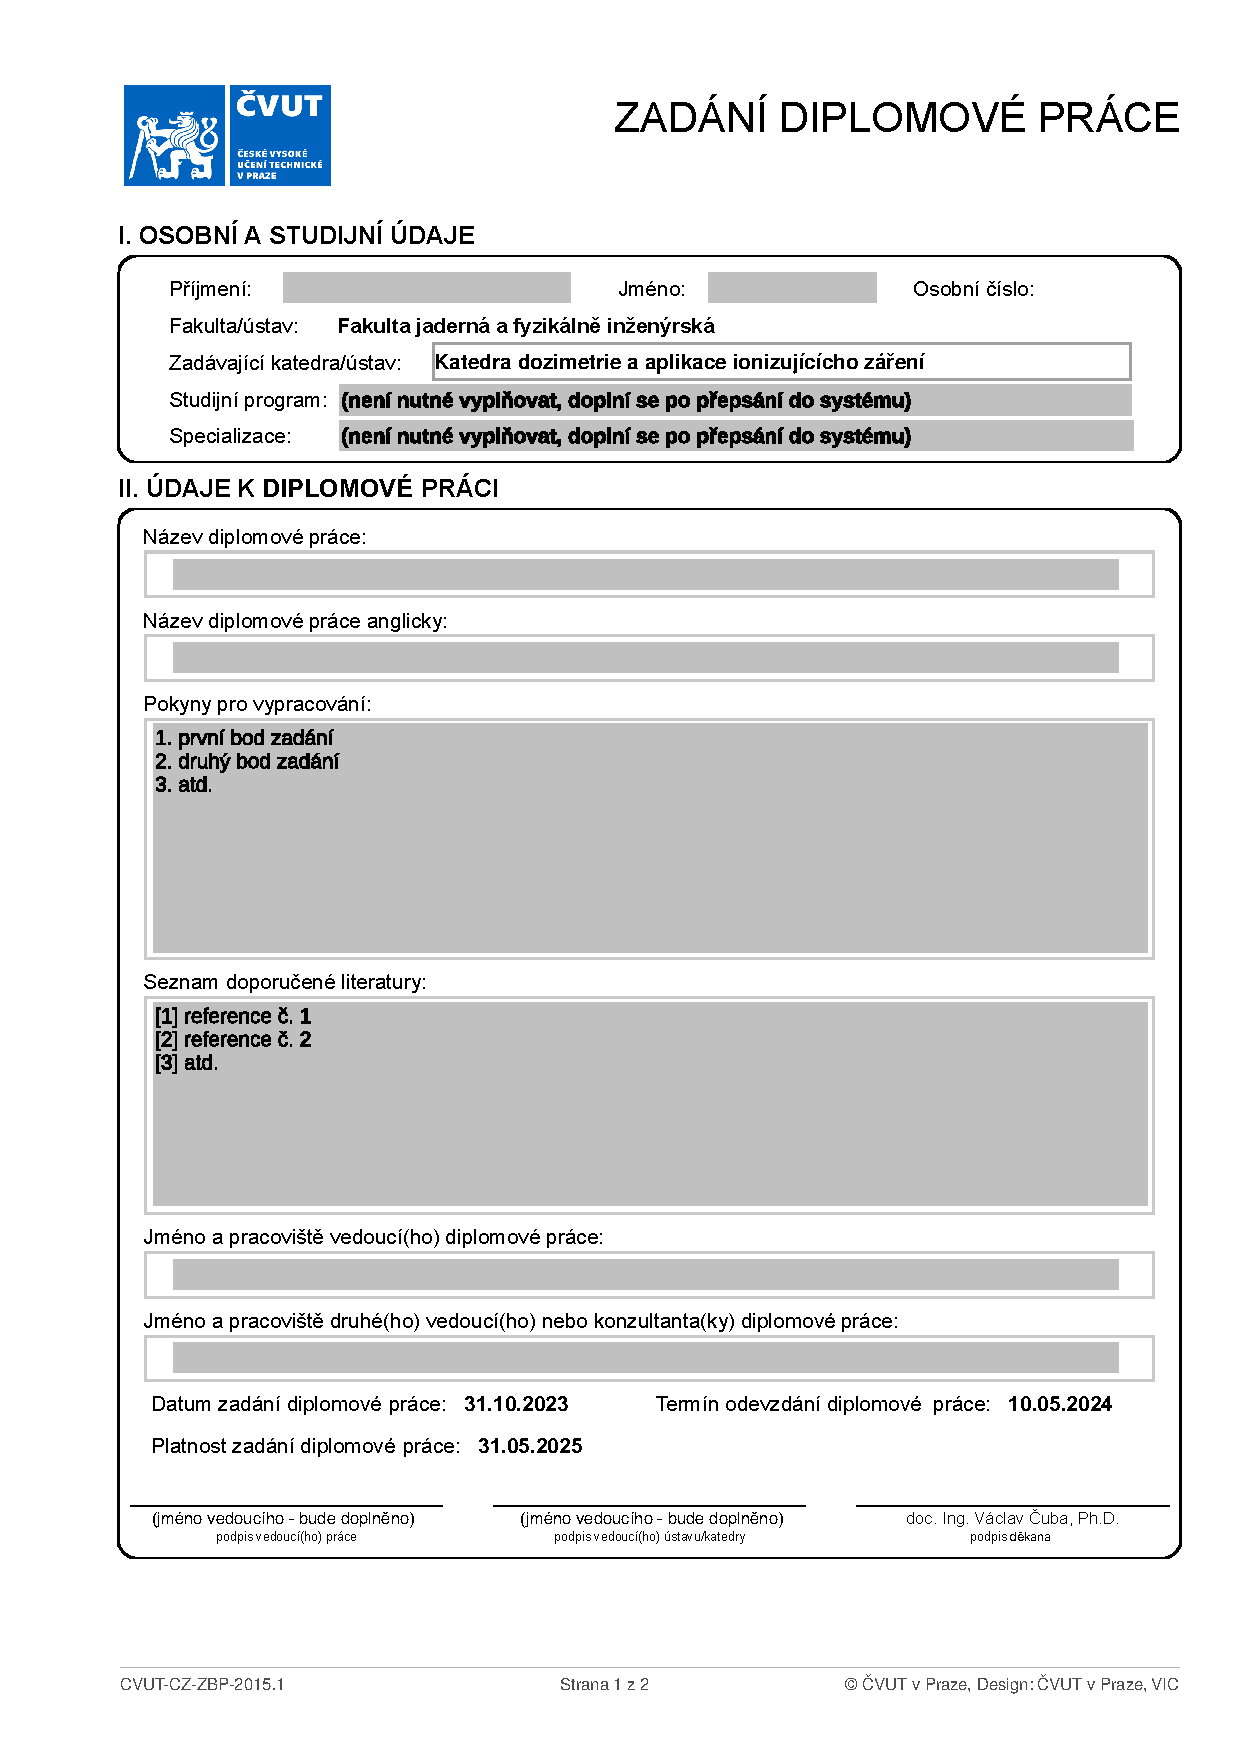
\includepdf[pages=-]{zadani.pdf}

\newpage 
\thispagestyle{empty}  

% Prohlášení si vygenerujete v KOSu
\newpage
\thispagestyle{empty}

\includepdf[pages=-]{prohlaseni.pdf}

% ---
\newpage
\thispagestyle{empty}

~
\vfill

{\bf \noindent Poděkování} 

\vspace{0.5cm} 
\noindent Ráda bych poděkoval/a\dots

Tento výzkum byl podpořen \dots

\begin{flushright}
\autor
\end{flushright} 

\newpage
\thispagestyle{empty}

{
	\setlength{\parindent}{0pt}
	
	\textit{Název práce:}
	\textbf{\nazevcz} \\
	
	\textit{Autor:} \autor \\
	
	\textit{Obor:} \obor \\
	
	\textit{Druh práce:} \typprace \\
	
	\textit{Vedoucí práce:}  \vedouci, \pracoviste \\
	
	\textit{Konzultant:}  \konzultant, \pracovistek \\ 
	
	\textit{Abstrakt:} 
	\abstrCZ \\
	
	\textit{Klíčová slova:}  \klicova
}

\newpage
\thispagestyle{empty}
{
	\setlength{\parindent}{0pt}
\textit{Title:}
\textbf{\nazeven} \\

\textit{Author:} \autor \\

\textit{Abstract:} 
\abstrEN \\

\textit{Keywords:}  \keywords
}
